\documentclass[../Cours.tex]{subfiles}

\begin{document}
\setcounter{chapitre}{19}
\chapitre{Quadrilatères}

\partie{Rectangle}
\definition{Un rectangle est un quadrilatère possédant 4 angles droits et des côtés opposés de même longueur.}

\illustration{
    \begin{center}
    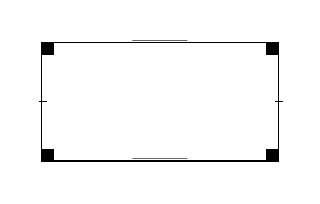
\begin{tikzpicture}
        \draw (0,0) -- (3,0) node[midway]{||} -- (3,1.5) node[midway]{\_} -- (0,1.5) node[midway]{||} -- cycle node[midway]{\_};
        \fill (0,0) rectangle +(0.15,0.15);
        \fill (3,0) rectangle +(-0.15,0.15);
        \fill (3,1.5) rectangle +(-0.15,-0.15);
        \fill (0,1.5) rectangle +(0.15,-0.15);
    \end{tikzpicture}
    \end{center}
}

\propriete{
    \begin{itemize}
        \item Les diagonales se coupent en leur milieu.
        \item Les diagonales sont de même longueur.
    \end{itemize}
    \begin{center}\color{noir}
        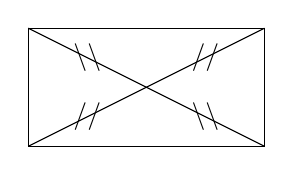
\begin{tikzpicture}
            \draw (0,0) rectangle (3,1.5);
            \draw (0,0) -- (1.5,0.75) node[midway]{//} -- (3,1.5) node[midway]{//};
            \draw (3,0) -- (1.5,0.75) node[midway]{\textbackslash\textbackslash} -- (0,1.5) node[midway]{\textbackslash\textbackslash};
        \end{tikzpicture}
    \end{center}
}

\clearpage
\partie{Losange}

\definition{Un losange est un quadrilatère dont les 4 côtés sont de même longueur.}

\illustration{
    \begin{center}
        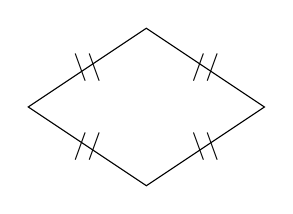
\begin{tikzpicture}
            \draw (0,0) -- (1.5,1) node[midway]{\textbackslash\textbackslash} -- (3,0) node[midway]{//} -- (1.5,-1) node[midway]{\textbackslash\textbackslash} -- cycle node[midway]{//};
        \end{tikzpicture}
    \end{center}
}

\propriete{
    \begin{itemize}
        \item Les diagonales se coupent en leur milieu.
        \item Les diagonales sont perpendiculaires.
    \end{itemize}
    \begin{center}\color{noir}
        \begin{tikzpicture}
            \draw (0,0) -- (1.5,1) -- (3,0) -- (1.5,-1) -- cycle;
            \draw[rouge] (0,0) -- (1.5,0) node[midway]{||} -- (3,0) node[midway]{||};
            \draw[rouge] (1.5,1) -- (1.5,0) node[midway]{\_} -- (1.5,-1) node[midway]{\_};
            \fill[rouge] (1.5,0) rectangle +(0.15,0.15);
        \end{tikzpicture}
    \end{center}
}

\partie{Carré}

\definition{Un carré a 4 côtés égaux et 4 angles droits.}

\propriete{Le carré a les mêmes propriétés que le losange \underline{et} le rectangle.}

\clearpage
\EXERCICES
\begin{questions}
    \exercice 
    \begin{center}
        \begin{tikzpicture}
            \draw (0,0) node[left]{$A$} -- (1.5,1) node[above]{$B$} -- (3,0) node[right]{$C$} -- (1.5,-1) node[below]{$D$} -- cycle;
            \draw[rouge] (0,0) -- (1.5,0) -- (3,0);
            \draw[rouge] (1.5,1) -- (1.5,0) -- (1.5,-1);
            \fill[rouge] (1.5,0) rectangle +(0.15,0.15);
        \end{tikzpicture}
    \end{center}

        \question Démontrer que $ABCD$ est un losange.
        \question Si $AC=BD$, quelle est la nature de $ABCD$ ? Le démontrer.

    \exercice 
        \begin{center}
        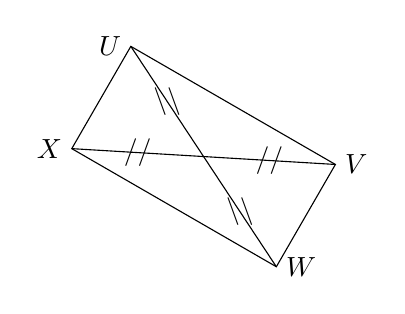
\begin{tikzpicture}[rotate=-30]
            \draw (0,0) rectangle (3,1.5);
            \draw (0,0) node[left]{$X$} -- (1.5,0.75) node[midway]{//} -- (3,1.5) node[right]{$V$} node[midway]{//};
            \draw (3,0) node[right]{$W$} -- (1.5,0.75) node[midway]{\textbackslash\textbackslash} -- (0,1.5) node[left]{$U$} node[midway]{\textbackslash\textbackslash};
        \end{tikzpicture}
        \end{center}

        \question Démontrer que $UVWX$ est un rectangle.
        \question Si $(UW) \perp (XV)$, quelle est la nature de $UVWX$ ?

    \exercice 
        \question Montrer que $IJKL$ est un carré.
        \question Calculer $IK$.
        \question Montrer que $(IK)\perp (LJ)$.
\end{questions}

\end{document}